\chapter{Dataset and Annotation}

This chapter describes the AI-CRAS dataset that forms the basis of all experiments, the ambiguity annotations added to it, and the statistical properties that motivate the experimental design.

\section{The AI-CRAS Dataset}

The experiments use the dataset introduced by Casalicchio and Cotumaccio \cite{casalicchio2024aicras}. It consists of 2,267 sentences extracted from publicly available Request for Proposal (RFP) documents related to cloud procurement and supplemented with seven synthetically generated documents produced via GPT-4 to increase domain coverage. Each sentence was independently examined by two annotators and classified along two dimensions.

First, a binary label indicates whether the sentence constitutes a cloud requirement (\texttt{goal = 1}) or not (\texttt{goal = 0}). Second, a set of six one-hot encoded indicators assigns the sentence to one or more cloud service categories, following the AI-CRAS ontology described in Chapter~2: \texttt{compute}, \texttt{data\_handling}, \texttt{network}, \texttt{security\_compliance}, \texttt{management\_monitoring}, and \texttt{cloud\_service\_essentials}. The assignment is multi-label: a single sentence can carry zero, one, or several categories. Disagreements between the two annotators led to exclusion of the disputed sample, preserving consistency.

\section{Ambiguity Annotation}

To support the experiments, each sentence in the dataset was manually annotated for ambiguity. The annotation follows the five-way taxonomy established by Berry and systematised by Bano \cite{bano2015ambiguity}, introduced in Chapter~2. Two columns were added:

\begin{itemize}
    \item \texttt{ambuiguity}: binary, set to 1 if the sentence exhibits any form of ambiguity and 0 otherwise.
    \item \texttt{ambiguity\_type}: integer encoding the specific type, with values 1--5 corresponding to lexical, syntactic, semantic, language-error, and pragmatic ambiguity respectively. A value of 0 indicates no ambiguity.
\end{itemize}

The annotation was conducted in a single pass: each sentence received exactly one type label, corresponding to the dominant form of ambiguity present. The five types are defined as follows, with representative examples drawn from the dataset:

\begin{description}
    \item[Lexical ambiguity] (type 1). A word or phrase conveys multiple meanings depending on context. \textit{Example:} ``The database server storage has to be provided on high speed disks (SSD's) for better performance'' — ``high speed'' and ``better performance'' are qualitative terms that admit no single quantitative interpretation. In procurement documents, lexical ambiguity is pervasive: terms such as ``adequate'', ``high availability'', ``fast response'', and ``scalable'' recur without numerical bounds.

    \item[Syntactic ambiguity] (type 2). The grammatical structure admits more than one valid parse. \textit{Example:} ``CSP / Bidder to conduct vulnerability assessment scanning of the Portal/Website for every 1 hour till the website is LIVE for rendering services'' — the modifier ``for every 1 hour'' could attach to ``scanning'' or to ``LIVE'', yielding different obligations.

    \item[Semantic ambiguity] (type 3). The logical content supports multiple interpretations even when the syntax is clear. \textit{Example:} ``It is the prime responsibility of CSP to ensure continuity of service at all times of the Agreement including exit management period (may be one month)'' — the phrase ``at all times'' conflicts with the parenthetical ``may be one month'' without clarifying which constraint takes precedence.

    \item[Language-error ambiguity] (type 4). Grammatical mistakes or typographical errors obscure the intended meaning. \textit{Example:} ``All the equipment's/Devices in the path have to be in HA mode'' — the spurious apostrophe in ``equipment's'' suggests a typo rather than a possessive, and the acronym ``HA'' is left undefined, making the specification ambiguous.

    \item[Pragmatic ambiguity] (type 5). The meaning depends on implicit context not present in the text. \textit{Example:} ``This will include system maintenance windows'' — without a definition of what constitutes a maintenance window (duration, frequency, permitted downtime), the requirement is underspecified and cannot be verified.
\end{description}

Each example illustrates the connection between the abstract taxonomy and the concrete challenges of the dataset: the ambiguity is not theoretical — it arises from the way requirements are actually written in procurement documents, and it directly affects whether a classifier can reliably determine what the sentence is asking for.

\section{Dataset Statistics}

Of the 2,267 sentences, 689 (30.4\%) are annotated as ambiguous. The breakdown by ambiguity type is shown in Table~\ref{tab:ambiguity_distribution}.

\begin{table}[h]
\centering
\caption{Distribution of ambiguity types.}
\label{tab:ambiguity_distribution}
\begin{tabular}{lcc}
\toprule
Ambiguity Type & Count & \% of Ambiguous \\
\midrule
Lexical          & 581 & 84.3\% \\
Pragmatic        & 61  &  8.9\% \\
Semantic         & 28  &  4.1\% \\
Language-error   & 17  &  2.5\% \\
Syntactic        &  2  &  0.3\% \\
\midrule
Total ambiguous  & 689 & 100\% \\
\bottomrule
\end{tabular}
\end{table}

Lexical ambiguity dominates, accounting for over four-fifths of all ambiguous sentences. This is a direct consequence of RFP language: qualitative terms such as ``high speed'', ``adequate load balancers'', and ``better performance'' are routinely used without quantitative specification. Syntactic ambiguity is the rarest, consistent with the formal, template-driven style typical of procurement documents.

Ambiguity is not uniformly distributed across the six categories. Figure~\ref{fig:ambiguity_by_category} visualises the breakdown, and Table~\ref{tab:ambiguity_rate} reports the per-category rates.

\begin{figure}[htbp]
\centering
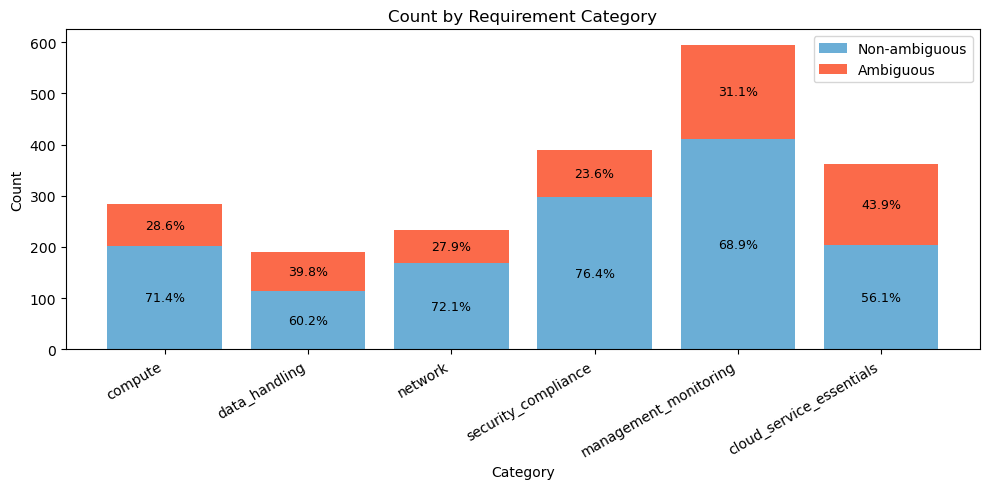
\includegraphics[width=0.85\textwidth]{figures/3_4.png}
\caption{Stacked breakdown of ambiguous and non-ambiguous sentences per cloud service category.}
\label{fig:ambiguity_by_category}
\end{figure}

\begin{table}[h]
\centering
\caption{Proportion of ambiguous sentences per category.}
\label{tab:ambiguity_rate}
\begin{tabular}{lccc}
\toprule
Category & Ambiguous & Total & Rate \\
\midrule
Cloud Service Essentials  & 159 & 362 & 43.9\% \\
Data Handling             &  76 & 191 & 39.8\% \\
Management \& Monitoring  & 185 & 595 & 31.1\% \\
Compute                   &  81 & 283 & 28.6\% \\
Network                   &  65 & 233 & 27.9\% \\
Security \& Compliance    &  92 & 390 & 23.6\% \\
\bottomrule
\end{tabular}
\end{table}

Cloud Service Essentials and Data Handling exhibit the highest ambiguity rates (43.9\% and 39.8\%), suggesting that requirements related to foundational cloud properties and data management are particularly prone to vague and underspecified phrasing. Security \& Compliance requirements are the least ambiguous (23.6\%), likely because security-related clauses in procurement documents tend to reference specific standards and certifications, which reduces vagueness.

The LLM-deambiguified variant of this dataset — in which every ambiguous sentence is rewritten with concrete clarifications — is generated from the annotated corpus using the procedure described in Chapter~4. It forms a parallel dataset that enables direct comparison of BERT's performance on original and disambiguated inputs.
